\documentclass[conference]{IEEEtran}
\IEEEoverridecommandlockouts
% The preceding line is only needed to identify funding in the first footnote.If that is unneeded, please comment it out.
\usepackage{cite}
\usepackage{amsmath,amssymb,amsfonts}
\usepackage{algorithmic}
\usepackage{graphicx}
\usepackage{textcomp}
\usepackage{xcolor}
\usepackage[utf8]{inputenc}
\usepackage[greek,english]{babel}
\usepackage{alphabeta}
\usepackage {hyperref}
\usepackage{makecell}
\usepackage{float}
\def\BibTeX{{\rm B\kern-.05em{\sc i\kern-.025em b}\kern-.08em
    T\kern-.1667em\lower.7ex\hbox{E}\kern-.125emX}}
\begin{document}

\title{Ασύρματα Δίκτυα με Χρήση Ορατού Φωτός\\}

\author{\IEEEauthorblockN{Ερρίκος Καλτσόπουλος}
\IEEEauthorblockA{\textit{Τμήμα Πληροφορικής Και Ηλεκτρονικών Συστημάτων} \\
Θεσσαλονίκη, Κεντρική Μακεδονία,Ελλάδα \\
ekal638@gmail.com}
}

\maketitle
%\renewcommand{\abstractname}{Περίληψη}

\begin{abstract}
Στο παρόν άρθρο αρχικά θα κάνουμε μια εισαγωγή για τα ασύρματα δίκτυα με τη χρήση του ορατού φωτός.Έπειτα θα γίνει αναφορά στα ιδιαίτερα χαρακτηριστικά,τις προκλήσεις και  τα πλεονεκτήματα.Στην συνέχεια θα επεκταθούμε στις εφαρμογές όπου τα χρησιμοποιούν η επωφελούνται από την χρήση τους.Τέλος , θα εστιάσουμε σε μια εφαρμογή και θα αναφερθούμε στα πλεονεκτήματα της  και στην αρχιτεκτονική της.
\end{abstract}

\begin{IEEEkeywords}
 Ασύρματα Δίκτυα με Χρήση Ορατού Φωτός, εφαρμογές, χαρακτηριστικά, προκλήσεις,πλεονεκτήματα,αρχιτεκτονική,λειτουργία,φυσικό
επίπεδο,επίπεδο ελέγχου πρόσβασης μέσου
\end{IEEEkeywords}

\section{Εισαγωγή}

\cite{b1}Τα ασύρματα δίκτυα με τη χρήση ορατού φωτός(vlc) χρησιμοποιούν το ορατό φως  σαν μέσο επικοινωνίας το οποίο καταλαμβάνει το φάσμα από 380nm εώς 750nm το οποίο αντιστοιχεί σε φάσμα συχνοτήτων 430Thz εώς 790Thz.Οι λάμπες που χρησιμοποιούνται είναι λάμπες φθορισμού με ταχύτητα μετάδοσης 10kbit/s η Led για 500mbit/s σε μικρές αποστάσεις .Το vlc  παρέχει μεγάλο έυρος ζώνης σε σχέση με το RF*.Επίσης για να λάβει σήματα ο δέκτης πρέπει να βρίσκετε στο ίδιο δωμάτιο με τον πομπό  αλλιώς δεν  θα μπορεί να λάβει κανένα σήμα έξω απο το δωμάτιο επομένως είναι και αρκετά ασφαλές.Ακόμη το vlc μπορεί να χρησιμοποιηθεί σαν πηγή φωτός πέρα από μέσο επικοινωνίας έτσι είναι και πιο οικονομικό σε σχέση με το RF.Λόγω των παραπάνω χαρακτηριστικών φαίνεται πολλά υποσχόμενο.

{\footnotesize \textsuperscript{*}Radio frequency (RF) Eίναι  ηλεκτρομαγνητικό κύμα το οποίο κυμαίνεται από 3 kHz έως  300 GHz.Το οποίο χρησιμοποιείτε για σήματα επικοινωνίας η ραντάρ}

\begin{figure}[h]
  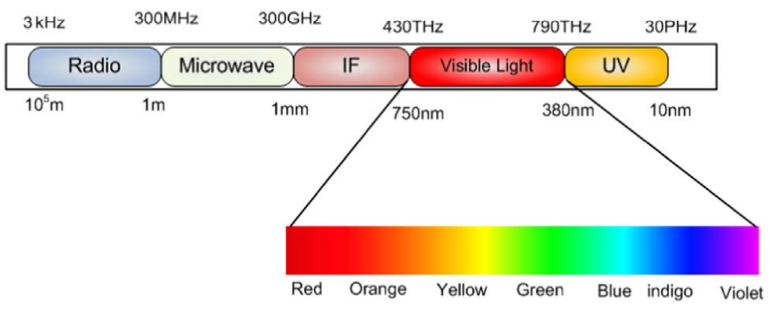
\includegraphics[width=\linewidth]{1.png}
  \caption{VLC φάσμα συχνοτήτων.}
 
\end{figure}

\section{Ασύρματα Δίκτυα με Χρήση Ορατού Φωτός}

\subsection{Ιδιαίτερα χαρακτηριστικά Δικτύων με τη χρήση ορατού φωτός \cite{b7}}

\begin{itemize}
\item Περιορισμός σήματος: 
Η φύση του φωτός είναι ότι δεν μπορεί να περάσει από αδιαφανείς τοίχους.Αυτό διευκολύνει τον περιορισμό των σημάτων σε ένα δωμάτιο, το οποίο αυξάνει το επίπεδο ασφάλειας του δικτύου.

\item Χωρίς οπτικό πεδίο: 
Επειδή τα συστήματα VLC χρησιμοποιούν το  φως σαν μέσο μετάδοσης, κάθε εμπόδιο μπορεί να αποτρέψει  την ικανότητά του να μεταδίδει δεδομένα.Αυτό όμως δεν ισχύει, καθώς δεν εξαρτάται από την οπτική γωνία.Στην πραγματικότητα, μελέτες έχουν δείξει ότι μπορούν ακόμα να αποδώσουν σε δωμάτια που έχουν σοβαρά εμπόδια.

\item Ασφαλές σε επικίνδυνα περιβάλλοντα:
Το VLC μπορεί να χρησιμοποιηθεί σαν εναλλακτική λύση για περιοχές όπου τα σήματα RF θεωρούνται ως επικίνδυνα.Εκτός από τη χρήση τεχνολογίας εκτός RF για την παράδοση δεδομένων, η πηγή φωτός που χρησιμοποιείται σε αυτά τα συστήματα εκπέμπει χαμηλές ενέργειες, διασφαλίζοντας την ασφαλή χρήση τους.Αυτά τα «επικίνδυνα» περιβάλλοντα περιλαμβάνουν νοσοκομεία, αεροπλάνα ή νάρκες.
\end{itemize}

\subsection{Προκλήσεις \cite{b5}}
To VLC είναι είναι πολλά υποσχόμενο μεσώ επικοινωνίας άλλα υπάρχουν κάποιες προκλήσεις που το απαρτίζουν:
\begin{itemize}
	\item  Ενσωμάτωση του VLC με την ήδη υπάρχουσα επικοινωνία πρότυπα όπως Wi-Fi κλπ.
	\item Το πρόβλημα της παρεμβολής σε πηγές φωτισμού περιβάλλοντος.
	\item  Αναμένεται παρεμβολή μεταξύ των διαφόρων συσκευών που χρησιμοποιούν VLC
γιατί στο  μέλλον θα  υπάρχει αύξηση του αριθμού των συσκευών VLC
	\item Περιορισμένο εύρος:
Το γεγονός ότι το φως δεν μπορεί να διεισδύσει στους τοίχους μπορεί να είναι καλό πράγμα όσον αφορά την ασφάλεια, αλλά αυτό σημαίνει επίσης ότι το VLC έχει πολύ περιορισμένο εύρος.Αυτό σημαίνει ότι μπορείτε να το χρησιμοποιήσετε αποτελεσματικά μόνο σε κλειστούς χώρους.Σε εγκαταστάσεις, τα φώτα πρέπει να τοποθετούνται τακτικά σε δωμάτια και αίθουσες για την επέκταση του πεδίου του δικτύου VLC.
	\item Περιορισμένη συμβατότητα
Δεδομένου ότι το VLC είναι μια νέα τεχνολογία, δεν είναι πολλές συσκευές συμβατές με αυτήν.Οι περισσότερες συσκευές που χρησιμοποιούμε τώρα εξακολουθούν να χρησιμοποιούν υλικό για δικτύωση Wi-Fi
\end{itemize}

\subsection{Πλεονεκτήματα \cite{b8}}

\begin{itemize}
\item Η επικοινωνία VLC λειτουργεί όταν τόσο η πηγή όσο και ο δέκτης βρίσκονται στο LOS(οπτικό πεδίο) εντός του ίδιου δωματίου.Η επικοινωνία δεδομένων με βάση το VLC δεν μπορεί να υποκλαπεί από κάποιον από το άλλο δωμάτιο.Ως εκ τούτου, το VLC παρέχει ασφαλή επικοινωνία σε αντίθεση με την επικοινωνία RF.


\itemΗ πηγή VLC χρησιμοποιείται τόσο για φωτισμό όσο και για επικοινωνία, έχει χαμηλή κατανάλωση ενέργειας.Επομένως  το VLC είναι ένα σύστημα εξοικονόμησης ενέργειας.


\item Το VLC είναι επικοινωνία με βάση το φως.παρόλα αυτά  δεν επηρεάζεται λόγω ακτινοβολιών από συστήματα RF.

\item Δεν έχει κινδύνους για την υγεία των ανθρώπων.

\item Είναι εύκολο στην εγκατάσταση.
\end{itemize}
\section{Εφαρμογές}


\subsection{Εφαρμογές που χρησιμοποιούν τα παραπάνω δίκτυα \cite{b1}}

\subsubsection{Li-Fi}
Το 2011 ο Γερμανός καθηγητής του πανεπιστημίου του Εδιμβούργου Harald Haas επινόησε τον όρο Light Fidelity(Li-Fi).Το (Li-Fi) είναι ένα υψηλής ταχύτητας ασύρματο δίκτυο το οποίο στηρίζεται στη χρήση ορατού φωτός και είναι συνδεδεμένο  αμφίδρομα ,χρησιμοποιείτε για  ασύρματη επικοινωνία  και είναι ανάλογο του Wi-Fi ,το οποίο χρησιμοποιεί  ράδιο συχνότητες για την επικοινωνία.Το πρόβλημα  με τα σήματα του wifi είναι ότι Παρεμβάλουν με πιλοτικά σήματα εξοπλισμού πλοήγησης σε αεροσκάφη.Όποτε για να αποτραπεί κάτι τέτοιο όπως και σε ανάλογες περιπτώσεις  τα Li-Fi φαίνεται να είναι μια καλή λύση.Το Li-Fi επίσης φαίνεται να παρέχει και υποστήριξη και στο Internet of Things (IoT).Οι ταχύτητες του Li-fi φτάνουν μέχρι τα 10Gbits/s η οποίες είναι 250 φορές περισσότερο από  μια πολύ γρήγορη ευρυζωνικη σύνδεση.

\subsubsection{Όχημα προς όχημα επικοινωνία}
Το VLC μπορεί να χρησιμοποιηθεί για επικοινωνία μεταξύ οχημάτων λόγω του ότι τα οχήματα έχουν ήδη φώτα μπρος και πίσω και υπάρχει η υποδομή.Οι εφαρμογές προτεραιότητας που υποδεικνύονται από το πρόγραμμα Επικοινωνιών Ασφάλειας Οχήματος περιλαμβάνουν προειδοποιητική προειδοποίηση σύγκρουσης μπροστά ,Ανίχνευση πριν από την σύγκρουση,Ηλεκτρονικά φώτα φρένων έκτακτης ανάγκης,Προειδοποίηση αλλαγής λωρίδας ,βοηθό αριστεράς στροφής, προειδοποίηση παραβίασης σήματος κυκλοφορίας και προειδοποίηση ταχύτητας.Όλες οι εφαρμογές πρέπει να είναι αξιόπιστες όταν πρέπει να παρέμβουν και να έχουν πολύ χαμηλό παράγοντα λάθους και λανθάνοντα χρόνο.Λόγω του ότι πρέπει να  έχουν πολύ χαμηλό λανθάνοντα χρόνο  στην επικοινωνία ασφάλειας του οχήματος  μπορεί να χρησιμοποιήθει  ένα σύστημα  επικοινωνίας  ορατού φωτός  υψηλής ταχύτητας όπως το Li-Fi.όπως φαίνεται στην Εικ.2.Στο \cite{b4}, ένα εξωτερικό σύστημα VLC που χρησιμοποιεί Controller Area Network (CAN) προτάθηκε και τα πίσω φώτα και οι προβολείς χρησιμοποιήθηκαν στο προτεινόμενο σύστημα επικοινωνίας.

\begin{figure}[h]
  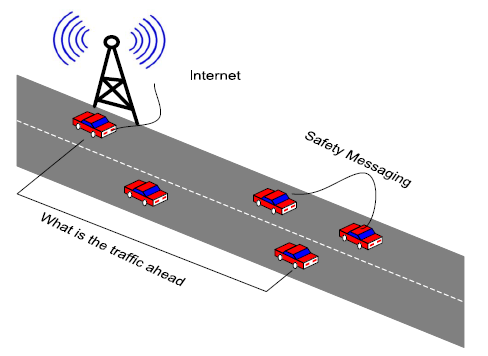
\includegraphics[width=\linewidth]{2.png}
  \caption{VLC για δίκτυο οχημάτων.} 
\end{figure}

\subsubsection{Έξυπνο σύστημα μεταφοράς \cite{b6}}
Έρευνες έχουν δείξει ότι πολλά από τα ατυχήματα που συμβαίνουν είναι λόγο της αργής ανταπόκρισης των οδηγών .Στο ITS  η επικοινωνία όχημα προς όχημα και υποδομης προς οχημα διασφαλίζει την ασφάλεια  και την άνεση των ανθρώπων.Το ΙΤS βασίζεται σε ασφαλή  και αξιόπιστη  επικοινωνία μεταξύ οχημάτων και υποδομών όπως  τα φανάρια και τις  πινακίδες.Όλα τα οχήματα είναι εξοπλισμένα με εμπρόσθια και πίσω φώτα που μπορούν να χρησιμοποιηθούν για τη μετάδοση πληροφοριών όπως είπαμε και παραπάνω.Φωτεινοί σηματοδότες ή πινακίδες μπορούν επίσης να χρησιμοποιηθούν για την ανταλλαγή χρήσιμων πληροφοριών σχετικά με το δρόμο, την κυκλοφορία και τις καιρικές συνθήκες.

\begin{figure}[h]
  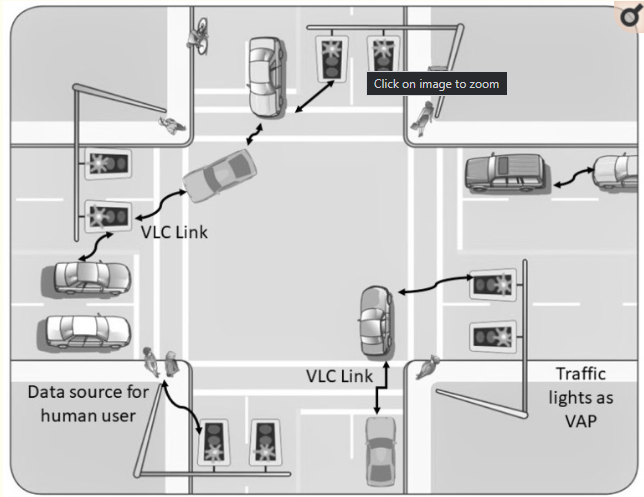
\includegraphics[width=\linewidth]{8.png}
  \caption{Ένα έξυπνο σύστημα μεταφοράς που χρησιμοποιεί την επικοινωνία ορατού φωτός.} 
\end{figure}

\subsubsection{Υποβρύχια επικοινωνία}
Τα κύματα RF δεν μεταδίδονται  καλά στο θαλασσινό νερό λόγω της καλής αγωγιμότητας του.Επομένως, η επικοινωνία VLC  μπορει  να χρησιμοποιείται σε υποβρύχια δίκτυα επικοινωνίας.Το Un Tethered Remote Operated Vehicle (UTROV) είναι μια άλλη εφαρμογή του VLC στην υποβρύχια επικοινωνία.Οι διάφορες εργασίες που μπορούν να εκτελεστούν χρησιμοποιώντας το UTROV περιλαμβάνουν τη συντήρηση των εξερευνητικών σκαφών.Το Σχ. 4 περιγράφει τη λειτουργία του UTROV.Το δεξί παράθυρο δείχνει την επικοινωνία του UTROV χρησιμοποιώντας το οπτικό κανάλι σε μια σταθερή υποδομή στον πυθμένα της θάλασσας.Στο κέντρο, η επικοινωνία επιτυγχάνεται με το UTROV χρησιμοποιώντας ένα οπτικό κανάλι με υποδομή ρελέ στο πλοίο.Το αριστερότερο παράθυρο δείχνει την επικοινωνία του UTROV χρησιμοποιώντας χαμηλό εύρος ζώνης υποβρύχιες διαβιβάσεις.

\begin{figure}[h]
  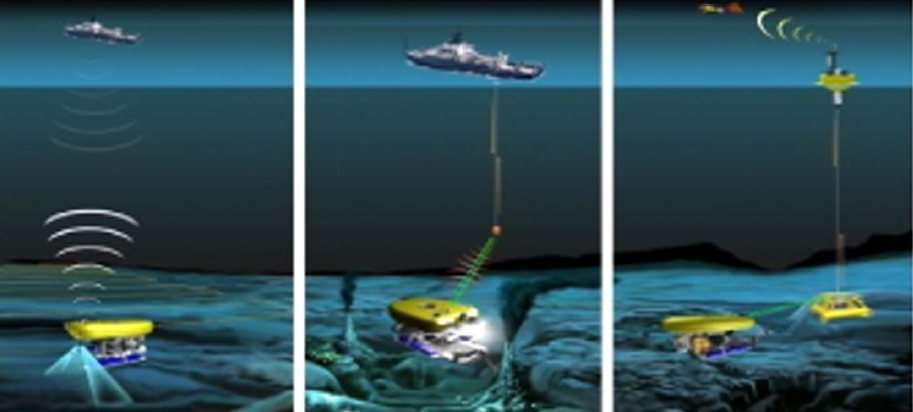
\includegraphics[width=\linewidth]{3.png}
  \caption{Λειτουργία του Ultrov.} 
\end{figure}

\subsubsection{Νοσοκομεία}
Στα νοσοκομεία, οι ευαίσθητες σε ηλεκτρομαγνητικά κύματα περιοχές (όπως οι σαρωτές μαγνητικής τομογραφίας) είναι πιθανό να μεταβούν σε VLC επειδή δεν θα επηρεάσει τα ραδιοκύματα των άλλων μηχανών.Ένα ρομπότ που ονομάζεται HOSPI (φαίνεται στο Σχ. 6) το οποίο  χρησιμοποιήθηκε  σε νοσοκομεία.Οι βελτιώσεις του συστήματος ελέγχου στο HOSPI έγιναν χρησιμοποιώντας VLC  το οποίο εγκαταστάθηκε  σε αισθητήρες του κτιρίου και στην πλοήγηση του ρομπότ.

\begin{figure}[h]
  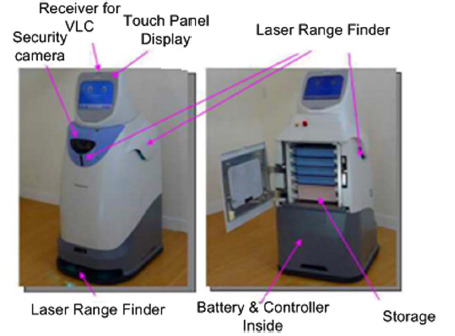
\includegraphics[width=\linewidth]{4.png}
  \caption{HOSPI.} 
\end{figure}

\subsubsection{Πληροφορίες που εμφανίζουν πινακίδες}
Οι πινακίδες κατασκευάζονται συχνά από μια σειρά LED που με τη σειρά τους διαμορφώνονται για να μεταφέρουν πληροφορίες σε αεροδρόμια, στάσεις λεωφορείων και άλλα
μέρη όπου είναι απαραίτητη η μετάδοση δεδομένων.Η πινακίδα μπορεί να χρησιμοποιηθεί για τη μετάδοση δεδομένων. Αυτός ο τύπος πινακίδας μπορεί να χρησιμοποιηθεί για ενδείξεις σε διάφορες τοποθεσίες όπως αεροδρόμια, μουσεία και νοσοκομεία.



\subsubsection{Visible light ID system}
 Το ορατό φως μπορεί να χρησιμοποιηθεί ως σύστημα ταυτότητας σε διαφορετικά μέρη, όπως κτίρια και υπόγειοι σιδηρόδρομοι.Για παράδειγμα, αν στεκόμαστε στο δωμάτιο 12 σε ένα συγκεκριμένο κτίριο.Ένα σύστημα αναγνώρισης ορατού φωτός μπορεί να χρησιμοποιηθεί για να προσδιορίσει τον αριθμό δωματίου και το κτίριό του.Παρομοίως, ένα σύστημα αναγνώρισης ορατού φωτός μπορεί να χρησιμοποιηθεί σε μετρό, νοσοκομεία και αεροδρόμια (Εικ. 7).

\begin{figure}[h]
  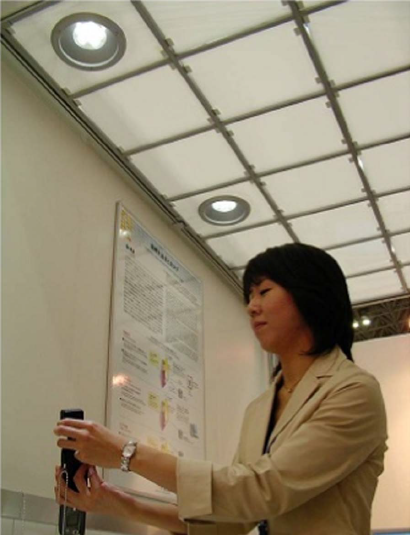
\includegraphics[width=\linewidth]{5.png}
  \caption{Πρωτότυπο που παρουσιάστηκε από την NEC και τη Matsushita Electric Works.} 
\end{figure}


\subsubsection{A Sound communication system}
Τα κόκκινα, πράσινα και μπλε LED χρησιμοποιούνται για τη μετάδοση μουσικών σημάτων.

\begin{figure}[h]
  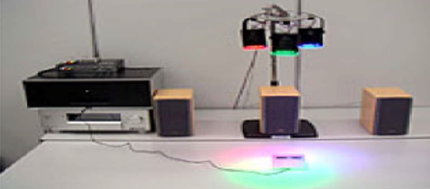
\includegraphics[width=\linewidth]{6.png}
  \caption{Το VLC σε να σύστημα μουσικής.} 
\end{figure}

\subsubsection{Wireless Local Area Networks (WLANs)}
Η επικοινωνία με ορατό φως με βάση LED μπορεί να χρησιμοποιηθεί για τη ρύθμιση LAN.Στο   Σχ. 8, προτείνεται ένα εξαιρετικά υψηλής ταχύτητας  αμφίδρομο, LAN βασισμένο στην αρχιτεκτονική τοπολογίας αστεριών που χρησιμοποιεί επικοινωνία ορατού φωτός LED για να παρέχει ταχύτητα μεγαλύτερη από 10Gb / s.Το σχηματικό διάγραμμα του LAN υψηλής ταχύτητας φαίνεται στο Σχ. 8.Ο λόγος για τη σχεδίαση του δικτύου χρησιμοποιώντας μια τοπολογία αστέρων είναι για παροχή υποστήριξης σε Πολλαπλούς χρήστες χρήστες.Η ίνα χρησιμοποιείται σε συνδυασμό με κάθε λαμπτήρα απευθείας όπως φαίνεται στο Σχ. 8.Το υβριδικό πρωτόκολλο πρόσβασης χρησιμοποιείται στο προτεινόμενο LAN, όπως και το Time Division Multiplexing (TDM)** για αμφίδρομη μετάδοση VLC και Frequency Division Multiplexing (FDM)** για μετάδοση uplink και downlink fiber.Τα αποτελέσματα του προτεινόμενου LAN  έδειξαν  την δυνατότητα  του να προσφέρει πρόσβαση υψηλής ταχύτητας σε πολλαπλούς χρήστες.

{\footnotesize \textsuperscript{**}Το TDM (Time Division Multiplexing) και το FDM (Frequency Division Multiplexing) είναι οι δύο τεχνικές πολυπλεξίας.Η κοινή διαφορά μεταξύ TDM και FDM είναι ότι το TDM μοιράζεται το χρονοδιάγραμμα για τα διαφορετικά σήματα.Ενώ το FDM μοιράζεται την κλίμακα συχνότητας για τα διαφορετικά σήματα.}



\begin{figure}[h]
  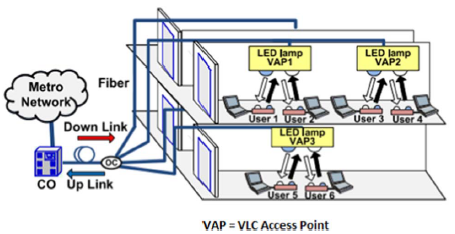
\includegraphics[width=\linewidth]{7.png}
  \caption{Το VLC δίκτυο σε σχηματικό διάγραμμα.\cite{b1}} 
\end{figure}

\subsection{Πλεονεκτήματα για μια συγκεκριμένη εφαρμογή \cite{b5}}
\begin{itemize}
	\item Ταχύτητα:
Τα κύματα φωτός είναι σε θέση να μεταφέρουν πολύ περισσότερες πληροφορίες από τα ραδιοκύματα που χρησιμοποιούνται στην τεχνολογία Wi-Fi, καθώς το φάσμα ορατού φωτός είναι σχεδόν 10.000 φορές μεγαλύτερο από το φάσμα που καταλαμβάνουν τα ραδιοκύματα.Αυτός είναι ο λόγος για τον οποίο η μετάδοση δεδομένων μέσω LiFi είναι 100 φορές ταχύτερη από τη μετάδοση δεδομένων μέσω Wi-Fi.Η σύνδεση LiFi μπορεί να μεταδώσει δεδομένα με ρυθμό 224 GB ανά δευτερόλεπτο.Σε αυτήν την ταχύτητα, μπορείτε να κατεβάσετε ένα βίντεο υψηλής ευκρίνειας σε δευτερόλεπτα!
	\item Αποδοτικότητα:
Το LiFi έχει τη δυνατότητα να είναι πιο ενεργειακά αποδοτικό και φθηνότερο λόγω της φύσης των λαμπτήρων LED που είναι ήδη αποδοτικοί από μόνοι τους.Η τεχνολογία LiFi τους δίνει έναν άλλο σκοπό, τη συνδεσιμότητα.Αυτό θα εξοικονομήσει κόστος σε σπίτια και χώρους εργασίας, διότι θα μπορούσε να γίνει χωρίς ηλεκτρονικές συσκευές, όπως δρομολογητές, μόντεμ, επαναλήπτες σήματος, ενισχυτές κυμάτων και κεραίες.Αυτές οι συσκευές πρέπει να είναι συνδεδεμένες στην τροφοδοσία 24/7 για να λειτουργούν.Το γεγονός ότι πολλές υποδομές πιθανότατα διαθέτουν ήδη φώτα LED, χρησιμοποιώντας το LiFi δεν θα ήταν επιπλέον κόστος.
	\item Ασφάλεια:
Τα ραδιοκύματα μπορούν να παρακολουθούνται από άτομα εκτός του δικτύου σας, καθώς μπορούν να περάσουν από τοίχους που θέτουν σε κίνδυνο την ασφάλεια των δεδομένων σας.Αλλά το φως σταματά από αδιαφανή αντικείμενα καθιστώντας το LiFi σημαντικά πιο ασφαλές από άλλες ασύρματες τεχνολογίες.
	\item Διαθεσιμότητα:
Με το LiFi, κάθε πηγή φωτός μπορεί να προσφέρει σύνδεση στο Διαδίκτυο.Στο εγγύς μέλλον, όταν η τεχνολογία είναι ήδη διαθέσιμη στο ευρύ κοινό, τα φώτα του δρόμου, τα φώτα κτιρίων και ο φωτισμός μεταφοράς μπορούν να επικοινωνούν ασύρματα και να έχετε πρόσβαση στο Διαδίκτυο όπου κι αν βρίσκεστε.
\end{itemize}
\section{Εφαρμογές}

\subsection{αρχιτεκτονική και η λειτουργία του δικτύου στo Li-Fi \cite{b9} }
Η αρχιτεκτονικη του Li-Fi αποτελειτε απο 3 σταδια .Τα 3 αυτα σταδια ειναι :Application Layer,Mac layer,physical Layer.Το IEEE 802.15.7 ορίζει μόνο δύο στάνταρ, δηλαδή το mac και physical layer  
\begin{figure}[h]
  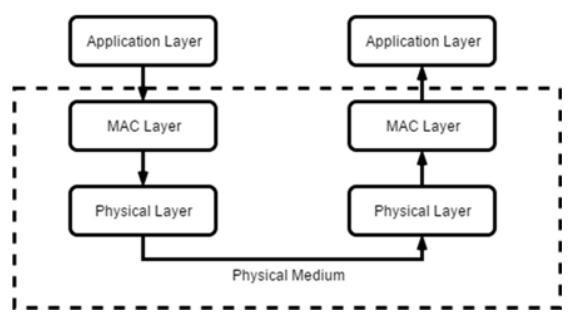
\includegraphics[width=\linewidth]{9.png}
  \caption{Αρχιτεκτονικη.} 
\end{figure}

\begin{itemize}
	\item Physical Layer
Το φυσικό επίπεδο είναι υπεύθυνο για τη μετάδοση και τη λήψη, την ενεργοποίηση και την απενεργοποίηση του οπτικού πομποδέκτη και την ανίχνευση της κατάστασης του καναλιού μετάδοσης, είναι σε κατάσταση αδράνειας ή μη.Υπάρχουν 3 τρόποι λειτουργίας στο φυσικό επίπεδο.Ο κάθε τρόπος λειτουργίας παρουσιάζετε στον Σχ. 10.
\begin{figure}[h]
  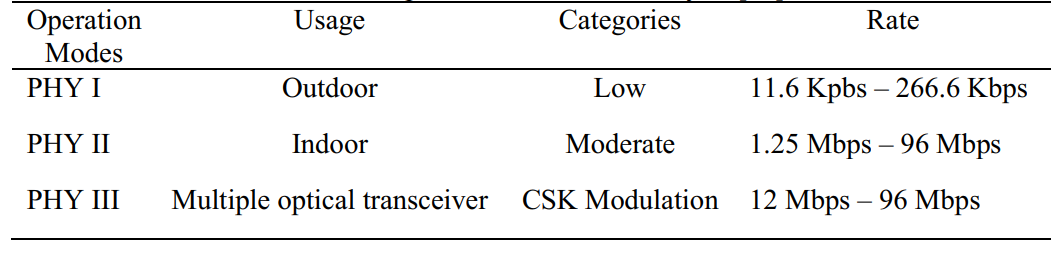
\includegraphics[width=\linewidth]{10.png}
  \caption{Οι 3 τρόποι λειτουργίας .} 
\end{figure}

\item MAC Layer
Τρεις τοπολογίες δικτύου ορίζονται στο επίπεδο MAC: Peer to peer, star και broadcast.
α) Peer to peer
Υπάρχουν δύο συσκευές που επικοινωνούν.Μια από αυτές είναι συντονιστής.
β) Star
Η επικοινωνία συμβαίνει σε πολλές συσκευές.Μια από αυτές είναι συντονιστής.
γ) Broadcast
Μία συσκευή, δηλαδή ένας συντονιστής στέλνει δεδομένα σε διάφορες συσκευές.Η επικοινωνία είναι μονόδρομη.

 \item Κανάλι διάδοσης
Το κανάλι διάδοσης στο LiFi δεν διαφέρει από το VLC.Το  εσωτερικό  του περιβάλλον χαρακτηρίζεται από έξι διαφορετικές διαμορφώσεις συνδέσμων οι συνδεσμοι των οποιων αναφερονται σε συνδέσμους IR*.Ο πομπός και ο δέκτης επικοινωνούν με δύο κριτήρια, δηλαδή άμεση ή έμμεση οπτική επαφή (LOS) που απαιτείται στο κανάλι διάδοσης.Αυτά τα δύο κριτήρια βασίζονται στον βαθμό κατεύθυνσης του πομπού και του δέκτη (LOS) άλλα βασίζονται στην ανάκλαση του φωτός (εκτός του LOS).Στο LOS οι σύνδεσμοι μεταξύ του πομπού και του δέκτη δείχνουν ή κατευθύνονται ο ένας τον άλλον.Ενώ στο non LOS το φως εξαπλώνεται από την αντανάκλαση της οροφής ή της επιφάνειας που αντανακλά.Το χαρακτηριστικό κάθε κριτηρίου συνοψίζεται στον Σχ. 11.

{\footnotesize \textsuperscript{*}Infrared  radiation (IR) Η υπέρυθρη ακτινοβολία είναι ηλεκτρομαγνητική ενέργεια σε μήκος κύματος ή μήκη κύματος κάπως μακρύτερη από εκείνη του κόκκινου φωτός.Το ασύρματο IR χρησιμοποιείται για επικοινωνίες μικρού και μεσαίου εύρους}

\begin{figure}[h]
  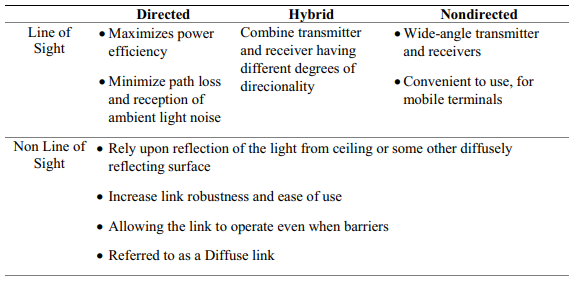
\includegraphics[width=\linewidth]{14.png}
  \caption{Χαρακτηριστικά του συνδέσμου  IR .} 
\end{figure} 
Η σημαντική παράμετρος για τη λήψη των υψηλών ποσοστών δεδομένων είναι η διαθεσιμότητα LOS.Μια μη απευθείας  μετάδοση LOS φαίνεται  να περιορίζει τους  ρυθμούς δεδομένων.


\end{itemize}
\subsection{Li-Fi vs WiFi σύγκριση ταχυτήτων}
Η αποτελεσματικότητα,ταχύτητα και η ασφάλεια του Διαδικτύου είναι τα κυρίαρχα ζητήματα για  την σημερινή εποχή.Ο σχεδιασμός του LiFi είναι να ξεπεράσει κάποια  μειονέκτημα του WiFi.Η ταχύτητα του WiFi είναι ένα από τα μειονεκτήματα που έρχεται να φέρει λύση το LiFi.Γιατί ίσως τα 1.3Gbps  ίσως δεν αρκούν σε κάποιες περιπτώσεις.Όπως βλέπουμε και στο Table I το WiFi έχει την δυνατότητα να φτάσει την μεγίστη ταχύτητα του 1.3Gbps με το 802.11ac Standard σε αντίθεση με το LiFi(Table II)  οπού μπορεί να φτάσει τα 3.4Gbps χρησιμοποιώντας  την διαμόρφωση DMT.Η ταχύτητα του LiFi μπορεί να είναι και  υψηλότερη από τα 3Gbps αλλά  η τεχνολογία βρίσκεται ακόμη υπό  έρευνα και ανάπτυξη.


\begin{table}[H]
\large
\caption{Speed of Li-Fi.\cite{b9}} % title of Table
\centering % used for centering table
\begin{tabular}{c c c} % centered columns (4 columns)
\hline\hline %inserts double horizontal lines
No & Modulation & Data Rate  \\ [0.5ex] % inserts table
%heading
\hline % inserts single horizontal line
1 & OOK & 803 Mbps \\ % inserting body of the table
2 & OFDM & 2.1 Gbps \\
3 & DMT & 3.4 Gbps  \\
4 & PPM & 30 Mbps  \\
5 & PAM & 20 Mbps  \\
6 & CAP & 1.1 Gbps  \\ [1ex] % [1ex] adds vertical space
\hline %inserts single line
\end{tabular}
\label{table:nonlin} % is used to refer this table in the text
\end{table}

\begin{table}[H]
\large
\caption{Speed and Standards of WiFi.\cite{b9}} % title of Table
\centering % used for centering table
\begin{tabular}{c c c} % centered columns (4 columns)
\hline\hline %inserts double horizontal lines
Standard & Release Date  & Max Speed  \\ [0.5ex] % inserts table
%heading
\hline % inserts single horizontal line
802.11b & 1999 & 11 Mbps \\ % inserting body of the table
802.11a & 1999 & 54 Mbps \\
802.11g & 2002 & 54 Mbps  \\
802.11n & 2007 & 72-600 Mbps  \\
802.11ac & 2013 & 433 Mbps -1.3 Gbps  \\ [1ex] % [1ex] adds vertical space
\hline %inserts single line
\end{tabular}
\label{table:nonlin} % is used to refer this table in the text
\end{table}

\subsection{Li-Fi vs WiFi Διαφορές}
Η σύγκριση του WiFi και του  LiFi έγινε βάση πολλών χαρακτηριστικών  όπως φαίνεται και στο Table III.Κάποια από αυτά αξίζει να σημειωθούν όπως: Ο δεκτής και  ο πομπός χρησιμοποιούν στο LiFi led ενώ στο   WiFi κεραία.Ο Αριθμός χρηστών που μπορούν χρησιμοποιήσουν το  LiFi είναι όσοι έχουν πρόσβαση στην λάμπα ενώ στο WiFi εξαρτάται από το Access Point άλλα δυστυχώς το εύρος κάλυψης είναι πολύ μικρο σε σχέση με το WiFi.Επίσης είναι πιο ασφαλές απο WiFi  επειδή το φως δεν μπορεί να περάσει από τοίχους.Το LiFi δεν έχει περιορισμούς στο που μπορεί  χρησιμοποιηθεί ενώ το WiFi δεν μπορεί να χρησιμοποιηθεί σε πχ αεροπλάνα και κάτω από το νερό. Τέλος έχει πολύ χαμηλή κατανάλωση ρεύματος όπως και επίπτωση στο περιβάλλον σε σχέση με το WiFi.


\begin{table}[H]
\footnotesize
\caption{Διαφορες Wifi - LiFi.\cite{b9}} % title of Table
\centering % used for centering table

\begin{tabular}{c c c} % centered columns (4 columns)
\hline\hline %inserts double horizontal lines
Parameter & LiFi  & WiFi \\ [0.5ex] % inserts table
%heading
\hline % inserts single horizontal line
Transmitter & LED  & Antenna \\  \hline% inserting body of the table
Receiver  & LED  & Antenna \\  \hline
Inbuilt Device & Under research and  development  & WiFi Card/Chip  \\ \hline
Average Operation Speed & Greater than 10Gbps (under research)  &150-600 Mbps  \\ \hline
Frequency band & 1000 times of THz & 2.4 GHz \\   \hline
Standard & IEEE 802.15.xx & IEEE 802.11xx  \\   \hline
No of users & All over under the lamp. & \makecell{Depend on\\ accesspoint.} \\   \hline
Data Transmission& Bits&Radio waves  \\   \hline
Coverage Area & 10 meters  & \makecell{20 – 100 meters \\varies based\\ on type of\\transmission power\\ and
antenna.}  \\   \hline
Interference &\makecell{No interference issues \\ with RF  waves}&
\makecell{Interference with \\neighbor AP routers}  \\   \hline
Topology & Point to Point & Point to Multipoint  \\   \hline
Communication & Based on VLC & \makecell{Based on\\Radio Frequency\\ Communication}  \\   \hline
Efficiency &\makecell{ More, LEDs \\consume less energy\\and highly efficient}&
\makecell{Less, Radio Base\\Stations consume\\high amount\\of energy}  \\   \hline
Availability & \makecell{Anywhere, available\\in airplanes \\and underwater}&Limited  \\   \hline
Secure&\makecell{More secure because\\light waves cannot\\penetrate through\\walls
and cannot\\be interceptby\\anyone outside the\\illumination of LED}&\makecell{Less secure \\because of high\\ penetrating power\\of \\radio waves,\\anyone can intercept } \\   \hline
NetWork Topology & Point to Point & Point to Multipoint  \\   \hline
Suitability & \makecell{Suitable for high\\ data rates and \\secure communication}&  \makecell{Suitable for\\ Aps with high\\ coverage regions} \\   \hline
Signal-to-Noise Ratio & Very high & Maybe more  \\   \hline
Power consumption &Less& More  \\   \hline
Environment Impact & Low  & Medium impact\\  [1ex]  \hline % [1ex] adds vertical space

\hline\hline %inserts single line

\end{tabular}
\label{table:nonlin} % is used to refer this table in the text
\end{table}

\begin{thebibliography}{00}
\bibitem{b1}https://www.sciencedirect.com/science/article/pii/S2352864816300335
\bibitem{b2}https://en.wikipedia.org/wiki/Visible\_light\_communication
\bibitem{b3}\href{https://www.researchgate.net/publication/290825448\_VLC\_technology\_for\_indoor\_LTE\_planning}{\nolinkurl{https://www.researchgate.net/publication/290825448}}
\bibitem{b4} D.-R. Kim, S.-H. Yang, H.-S Kim, Y.-H Son, S.-K Han, Outdoor visible light
communication for inter-vehicle communication using controller area network, in:
Proceddings of Fourth International Conference on the Communications and
Electronics (ICCE), 2012, pp.31-34.
\bibitem{b5}https://lifi.co/lifi-pros-cons/
\bibitem{b6}https://www.ncbi.nlm.nih.gov/pmc/articles/PMC6427442/
\bibitem{b7}https://lifi.co/visible-light-communication/
\bibitem{b8}https://www.rfwireless-world.com/Terminology/Advantages-and-Disadvantages-of-VLC-Visible-Light-Communication.html
\bibitem{b9}https://iopscience.iop.org/article/10.1088/1757-899X/325/1/012013/pdf 
\end{thebibliography}
\vspace{12pt}


\end{document}
